\documentclass{article}
\usepackage[nonatbib]{nips_2016}

\usepackage[breaklinks=true,letterpaper=true,colorlinks,citecolor=black,bookmarks=false]{hyperref}

\usepackage{amsthm}
\usepackage{amsmath,amssymb}
\usepackage{enumitem}

\usepackage[sort&compress,numbers]{natbib}
\usepackage[normalem]{ulem}

% use Times
\usepackage{times}
% For figures
\usepackage{graphicx} % more modern
%\usepackage{epsfig} % less modern
%\usepackage{subfig}

\graphicspath{{../fig/}}

\usepackage{tikz}
\usepackage{tkz-tab}
\usepackage{caption}
\usepackage{subcaption}
\usetikzlibrary{shapes.geometric, arrows}
\tikzstyle{arrow} = [very thick,->,>=stealth]

\usepackage{cleveref}
\usepackage{setspace}
\usepackage{wrapfig}
%\usepackage[ruled]{algorithm}
\usepackage{algpseudocode}
\usepackage[noend,linesnumbered]{algorithm2e}

\usepackage[disable]{todonotes}

\usepackage{algpseudocode}

\usepackage{amsmath}
\usepackage{booktabs}
\usepackage{multirow}
\usepackage{titlesec}

\newcommand{\red}[1]{\textcolor{red}{#1}}


\title{Dynamic Model Construction for Efficient Classification}

\author{
    Jaejun Lee \\
    School of Computer Science\\
    University of Waterloo\\
    Waterloo, ON, N2L 3G1 \\
    \texttt{j474lee@uwaterloo.ca} \\
}

\begin{document}
\maketitle

\begin{abstract}

One of the major drawback of neural network based classifier is that retraining is inevitable when target set of classes changes. For this reason, such networks are often designed to be wide and deep to support all possible classes. As a results, they are computationally expensive and can lead to unpleasant user experience. In this work, I propose Composing algorithm which allows dynamic construction of a classifier using class-level transfer learning. Composing algorithm does not require any extra computation but found to be less accurate once trained with cross entropy loss. I realize that sigmoid with binary cross entropy loss can minimize the accuracy decrease and evaluate how different loss function changes the behaviour of constructed model. After thorough experiments on MNIST, keyword spotting, and CIFAR-100, it is found that sigmoid with binary cross entropy loss is more suitable for Composing algorithm but decrease in accuracy is inevitable as number of classes increases.

\end{abstract}

\section{Introduction}

Over the last decade, neural network has became {\it de facto} approach for numerous classification problems as it leads to high accuracy~\cite{lecun1998gradient, chen2014small, krizhevsky2009learning}. However, neural network based approaches require much larger computation and less flexible than preexisting techniques. When training neural network based classifier, a set of target class must be provided in order to obtain reliable classifier. A trained model then can be deployed and classify unseen data assuming that true class of the given data belongs to target set which the model is trained on. However, in practice, this is not always the case and there exist two extreme cases where this setup falls apart.

The first case is when a set of true class contains only few classes from target class set. In this case, the trained model is considered to be an excessive representation of the true classifier and wastes the resources as it calculates probabilities for unnecessary classes. This can be avoid when a set of true class is known prior to training, by training the model to classify only the necessary classes.

The other case is when the true class of an unseen data does not exist in the target classes. Unless the model is explicitly trained to classify such class as unknown, the model will classify the unseen data to be one of target classes and such misclassification can lead to system failure. The ideal solution for this issues is to train a model again with the new class, minimizing the chance of misclassification.

However, training a neural network is a very expensive operation. It can take days to obtain reliable classifier and this hinders the efficient management of a service. To combat this issue, most of the academic works focus on minimizing resource usages of a network while preserving the highest accuracy. However, there exist an alternative solution to this problem: constructing a model dynamically adapting to the change in target set while minimizing decrease in accuracy and increase in resource usage. There are three conditions which the optimal solution must satisfy:

\begin{enumerate}
    \item \textbf{Minimal accuracy degradation} : the difference in accuracy between constructed model and the base model should be small
    \item \textbf{Dynamic class addition and removal} : it must be easy to add and remove a class from the constructed model
    \item \textbf{Efficient classification} : the constructed model should not require more computations than the base model
\end{enumerate}

In the above criteria, base model refers to a model which is trained explicitly to classify the same set of class as the constructed model.

It is found that dynamic model construction is quite challenging as the optimal solution requires a technique which considers relationship between each of the neurons and the output value for every class. In this paper, I present Composing algorithm which obtains such information by class-level transfer learning. As Composing algorithm involves mixing up the weights obtained from distinct models, I realize the limitation of standard cross entropy loss approach and show that sigmoid with binary cross entropy loss is more suitable for Composing algorithm. This has been demonstrated with a set of experiment as well. Conducted on MNIST, keyword spotting, and CIFAR-100, it is found that accuracy degradation is inevitable as number of classes increases but can be minimized when models are trained with sigmoid and binary cross entropy loss.

\section{Related Works}

Even though the three criteria for dynamic model construction are quite related, there exist distinct set of problems aiming to achieve each criteria. The three most relevant domains are: ensemble learning, multi-task learning, and transfer learning

\subsection{Ensemble Learning}
Ensemble learning is a common technique in the field of machine learning which achieves higher accuracy by combining outputs of multiple models. The most famous techniques include voting, weighting, bagging and boosting~\cite{dietterich2000ensemble, breiman1996bagging, freund1996experiments}. Even though ensemble learning is considered to be easy to implement, ensemble learning assumes that models are independent. As a result, most ensemble learning algorithms require each model to process the input data parallel violating the efficiency requirement of the dynamic model construction problem.

\subsection{Multi-task Learning}
On the other hand, multi-task learning takes the opposite approach; combine a set of networks to share the knowledge learned from each task. The key assumption is that if tasks are related, sharing knowledge throughout training will increase the performance of each network. Techniques for multi-task learning are often classified into two depending on the type of information being shared: parameter sharing and feature sharing~\cite{ruder2017overview, Caruana1993MultitaskLA, duong2015low, lu2017fully}. Its architecture and consideration of multi-tasks can be adapted to the dynamic model construction problem. However it fails to satisfy the efficiency requirements as most solutions have extra layers to share information among tasks without any modification to each model.

\subsection{Transfer Learning}

Transfer learning is inspired by the same assumption as multi-task learning; sharing knowledge among tasks can improve the performance. However, the key difference between two problems is that transfer learning use the same model architecture for different tasks. Transfer learning involves pre-training and fine-tuning. First, a model is pre-trained on a task and learns to select important features. Then the same model is fine-tuned for a target task as trained weights are adjusted to produce the best result for the target task~\cite{yosinski2014transferable}. It is found that transfer learning is very powerful as demonstrated in a wide range of problems~\cite{raina2007self, egan2004effects, glorot2011domain}. Unlike two aforementioned domains, transfer learning does not add any computations for the fine-tuned task. However, knowledge sharing is mostly studied on task-level and limited work exists for class-level transfer learning.

\section{Composing Algorithm}

In this section, I introduce Composing algorithm which enables dynamic model construction for efficient classification. I also discuss the necessary conditions to achieve the best accuracy from Composing algorithm.

\subsection{Approach}

\begin{figure*}[t!]
  \centering
  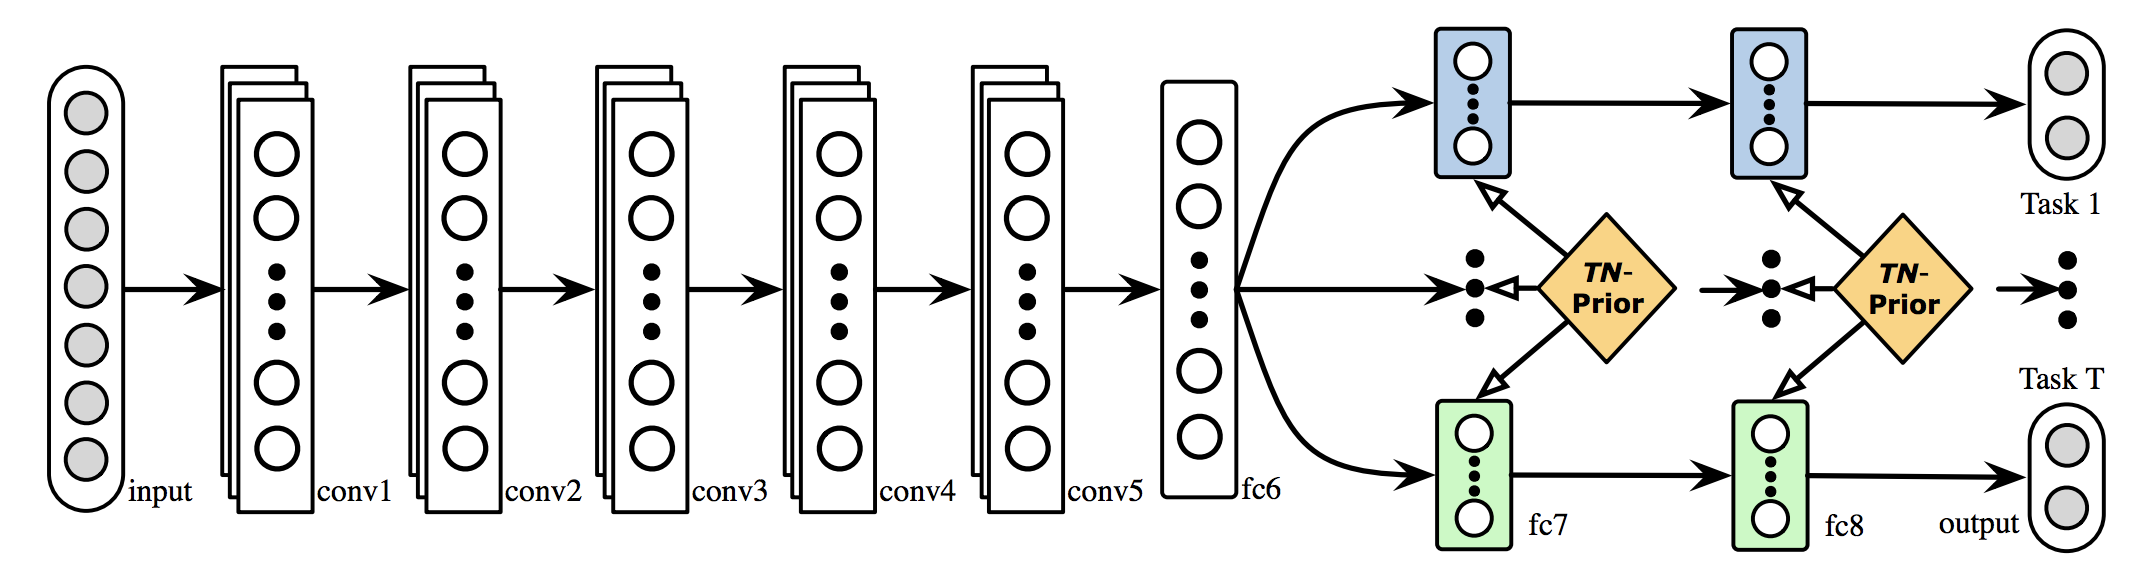
\includegraphics[scale=0.32,trim={0mm 0mm 0mm 0mm},clip]{long2017learning.png}
\end{figure*}

\begin{figure*}[t!]
	\centering
	\begin{subfigure}[b]{.65\linewidth}
		\centering
		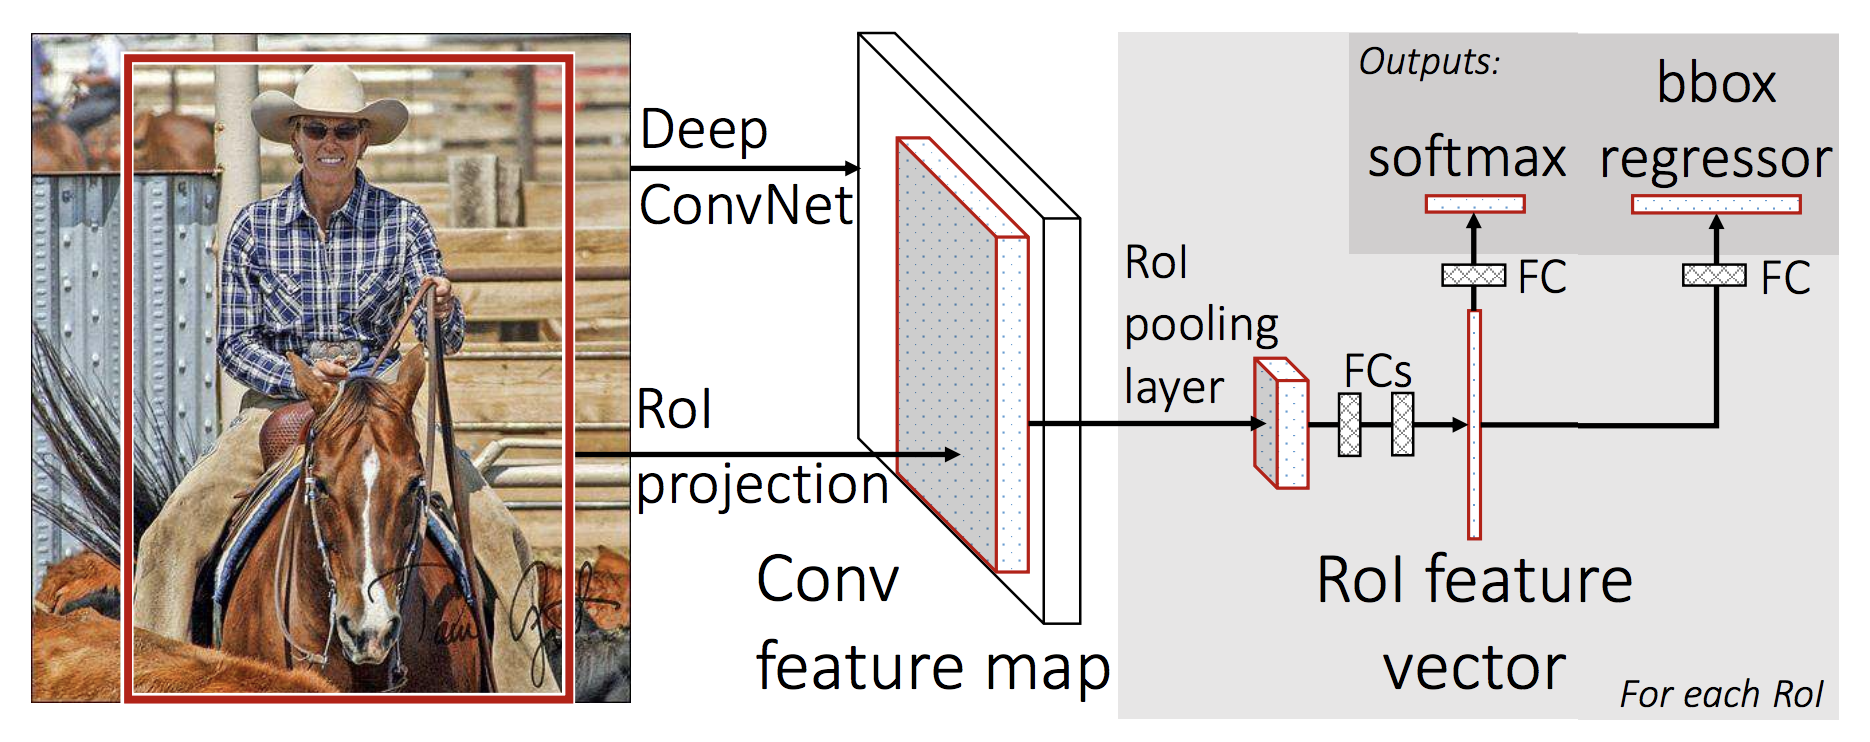
\includegraphics[scale=0.25,trim={0mm 0mm 0mm 0mm},clip]{girshick2015fast.png}
	\end{subfigure}%
	\begin{subfigure}[b]{.35\linewidth}
		\centering
		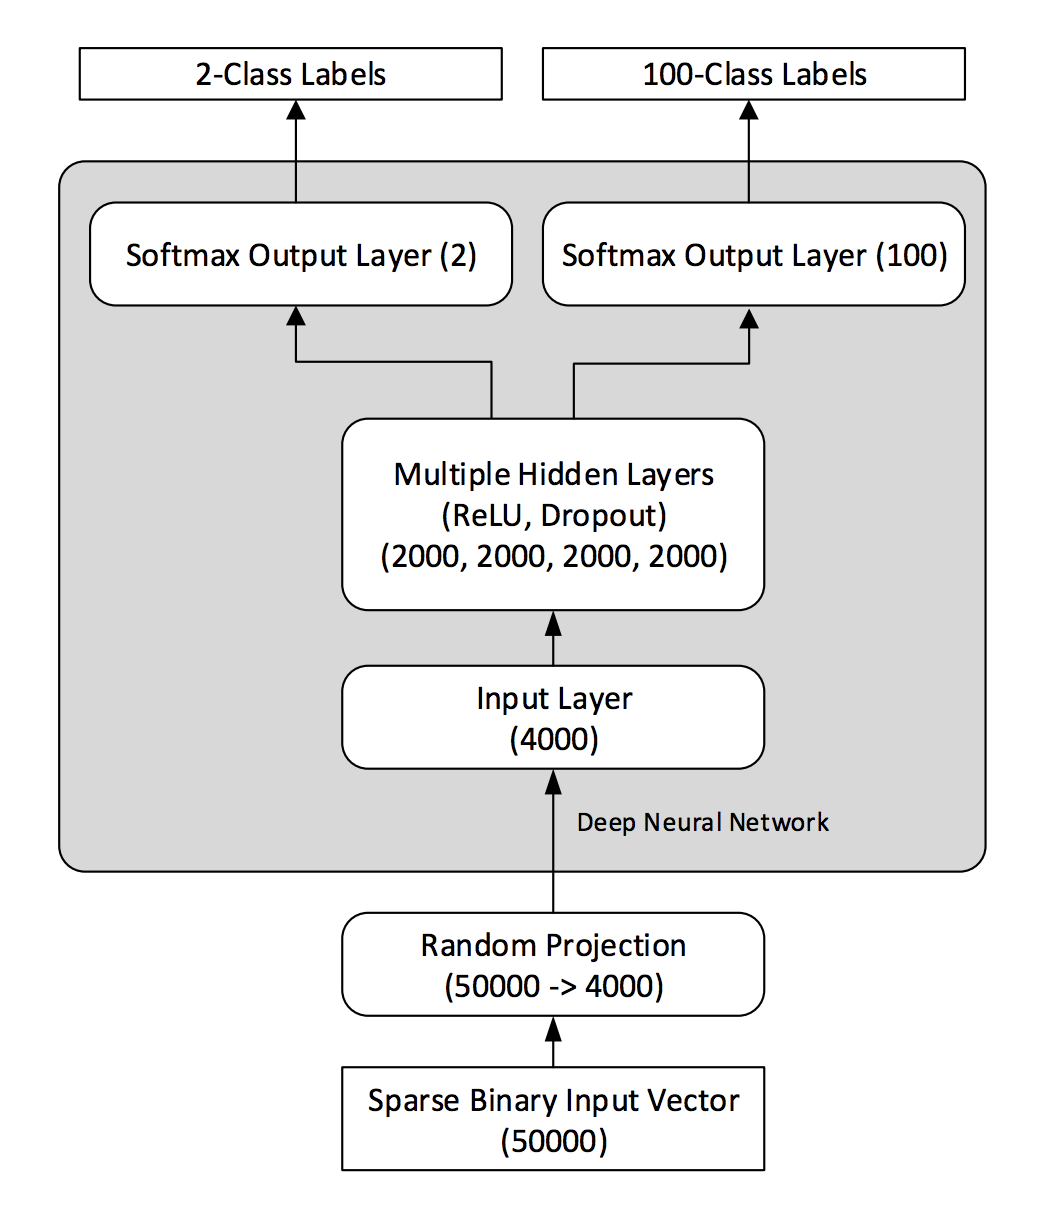
\includegraphics[scale=0.15,trim={0mm 0mm 0mm 0mm},clip]{huang2016mtnet.png}
	\end{subfigure}
	\caption{Model architectures proposed by ~\cite{long2017learning} (top), ~\cite{huang2016mtnet} (bottom right), and  ~\cite{girshick2015fast} (bottom left); Their approach for multi-task learning is to assign distinct fully-connected layer for each task.}
	\label{figure:mutli-task-learning}
\end{figure*}

One of the common approach for multi-task learning is to assign distinct fully-connected layer for each task (see Figure~\ref{figure:mutli-task-learning}). With such architecture, each task is trained independently while weights for upstream layers are shared among tasks. Once the training completes for the combined model, a task can be discarded from populating output by removing corresponding fully-connected layer.

Next, consider a case of transfer learning. It is found that pre-training a model and fine-tuning the model for target task can leads to increase in accuracy. There is no change in model architecture throughout this process. Therefore, fine-tuned model uses the same amount of computation as the model that is explicitly trained to accomplish the same task.

Recall the criteria for dynamic model construction. Above multi-task learning approach achieves the dynamic addition and removal of a class and transfer learning guarantees the necessary efficiency. Exploiting these two techniques in two different domains, the proposed algorithm has the following step:

\begin{enumerate}
    \item Pre-train a model as if it is multi-classification problem
    \item Freeze the model parameters
    \item Repeat step 4 $\sim$ 7 for each class
    \item Construct a dataset which labels target class as positive and the others as negative.
    \item Replace the last full-connected layer for two classes
    \item Fine-tune the last layer using the new dataset
    \item Retrieve class-specific weights (weights for positive class) of the fully-connected layer
    \item For every variation of target set, it is possible to construct corresponding model by replacing the last layer with the class-specific weights obtained from fine-tuning.
\end{enumerate}

For simplicity, I decide to call this algorithm as Composing algorithm, the model trained for multi-class as base model, models constructed from step 4 $\sim$ 7 as fine-tuned models and the model constructed from the last step as composed model.

Composing algorithm achieves dynamic addition and removal of a class by attaching and discarding corresponding fully-connected connections.
With such flexibility, retraining a classifier is no longer necessary. Furthermore, note that even though a class has not participated for step 1, it is possible to construct a composed model with that class as long as the same base model is used for fine-tuning.

When we are constructing a composed model, we only retrieve weights for positive class from each of fine-tuned model. Therefore, the composed model has exactly the same number of parameters with the base model. As a result, composing model does not violate the efficiency requirements.

\section{Accuracy Preservation}

However, does Composing algorithm also guarantees the minimal accuracy degradation between base model and composed model? To answer this question, we need to understand how different loss function affects the behaviour of the composed model.

\subsection{Limitations of cross entropy loss}

State of the art for multi-classification is to use cross entropy (CE) loss, which transforms output by applying softmax and calculates negative log likelihood (NLL) as a measure of loss. Consider the definition of CE loss and NLL loss:

\begin{align*}
NegativeLogLikelihood(y, t) & = -\frac{1}{N}\sum_{i=1}^N \left[ t_i \cdot \log y_i\right] \\
y_i = Softmax(x_i) &= \frac{e^{x_i}}{\sum_{j}e^{x_j}} \\
\end{align*}

where $x$ is the output of the network and $t$ is the target, one hot encoded vector as in common implementation. In other words, softmax calculates normalized logits of the network output. Therefore, $y$ has value between zero and one and they must sum up to one. Since multi-class classifier rely on the mutually exclusive assumption among target classes, CE loss is the most suitable as it promotes the positive class while suppressing the negative classes.

However, such assumption can lead to unpredictable behaviour with composing algorithm. When CE loss is used throughout the composing algorithm, the loss which used in fine-tuning is computed with respect to the output of negative class. However, for a composed model, probability for each class is computed using independently fine-tuned weights and a class with the highest probability is selected as a final prediction.

For example, let us say there are 3 classes: A, B, and C. For fine-tuning, each dataset is constructed with two classes: a positive class representing the target class and negative class representing all the other classes. For simplicity, positive weights are referred with lower case (a, b, and c) and negative weights with lower case with prime (a', b', and c'). During fine-tuning, loss is calculated in pairs: a -- a', b -- b', c -- c'. However, for composing step, the last layer consists of weights a, b and c. As a results, there is no guarantee that the class with the highest value is in fact the class with highest probability.

\subsection{Binary cross entropy with sigmoid}

Given that CE loss does not preserve the accuracy between the base model and composed model due to mutually exclusive assumption among classes, I propose binary cross entropy (BCE) loss with sigmoid to combat the accuracy degradation.

\begin{align*}
BinaryCrossEntropy(y, t) & = -\frac{1}{N}\sum_{i=1}^N \left[ t_i \cdot \log y_i + (1 - t_i) \cdot \log (1 - t_i) \right] \\
y_i = Sigmoid(y_i) &= \frac{1}{1 + e^{-x_i}} \\
\end{align*}

Unlike CE loss, both sigmoid and BCE loss treat each index independently. In other words, weights for each class obtained from fine-tuning does not depend on other classes. This indicates that class with the highest output from composed model is in fact most likely to be the true class among the target classes.

In multi-label classification, the same issue has been raised with CE loss~\cite{liu2017deep}. It is found that the independence guarantee provided by BCE loss with sigmoid is crucial for multi-label classification and enabled successful training of a classifier.

\section{Experiments}

Realizing the limitation of CE loss from the definitions, I have implemented Composing algorithm on MNIST, Keyword Spotting, and CIFAR-100 demonstrating its feasibility. Experiments are implemented with PyTorch and available on github\footnote{\url{https://github.com/ljj7975/composable-model-exp}}.

For each dataset, I construct a composed model using three different loss functions. First, I include CE loss. Since PyTorch NLL loss implementation expects log probability, log is applied after softmax but it is found that this does not affect the experiments. Next, I use sigmoid with BCE loss which is found to preserve accuracy better than CE loss. Last loss function is softmax with BCE loss. This setting is known to be unstable because BCE loss assumes the independence among classes while softmax does not. In fact, I have observed the training collapse at some point. However, as I report accuracy from the best model, I found the results from this setting still valid and meaningful. This setting should allow me to understand how crucial sigmoid is for sigmoid with BCE loss combination as it simply replace sigmoid with softmax.

Throughout the experiments, I report accuracy from every model created from Composing algorithm: base model, fine-tuned model, and composed model. Comparing accuracy of base model against corresponding composed model, it is possible to understand how stable Composing algorithm is with respect to each loss function.

In order to understand how the accuracy of composed model changes with respect to number of classes, I report accuracy from each intermediary composed model as I add a class to construct a composed model. Since fine-tuned accuracy for some classes are greater than the other, I repeat this step 10 times with randomly selection on next class to add and report average.

\subsection{MNIST}

MNIST is a standard benchmark for classification~\cite{lecun1998gradient} which consist of images for handwritten digits. Among the wide range of model architecture solving this problem, I have conducted my experiments with \texttt{LeNet-5}~\cite{lecun2015lenet}. \texttt{LeNet-5} is constructed with two convolutional, one dropout and two fully connected layers. The original implementation of \texttt{LeNet-5} has 10 and 20 channels for the first two convolutional layers and produces accuracy of 98\% on MNIST dataset. Since our goal of this experiment is to understand the change in accuracy as different loss functions are used for Composing algorithm, I intentionally limited the expressive power of the network by reconstructing the network with only 5 channels for both convolutional layers.

Both base model and fine-tuned models are trained using Adam optimizer with learning rate of 0.0001. After conducting 50 experiments, it is found that all three loss function converges to similar accuracy within 5 epochs. The base models converge to average accuracy of 95\% and fine-tuned models converge to 98\% (see Figure \ref{table:mnist}).

Table \ref{figure:composed_mnist} summarizes how the accuracy changes as number of classes increases for composed model. No matter which loss function is used for Composing algorithm, accuracy of composed model decreases as more classes contributes to the composed model. However, models with softmax based loss is found to suffer at a greater rate than models with sigmoid based loss. With CE loss, the composed model for all 10 classes has an accuracy of 85.86\% with relative decrease of 10.5\% from the base model accuracy. Composed model trained with softmax with BCE loss is found to be the worst. The average final accuracy is 78.50\% which is 17.85\% relative decrease. As expected, sigmoid with BCE loss introduces minimal accuracy degradation and achieves 95.29\% accuracy which is very similar to the base model accuracy.

\begin{table}[t]
    \centering
    \begin{tabular}{ccccccc}
        \toprule[1pt]
        \multirow{2}{*}{\raisebox{-3\heavyrulewidth}{\bf Loss function}} &
        \multirow{2}{*}{\raisebox{-3\heavyrulewidth}{\bf Base model}} &
        \multicolumn{3}{c}{\bf Fine tuned model } &
        \multicolumn{2}{c}{\bf Composed model } \\
        \cmidrule(lr){3-5}
        \cmidrule(lr){6-7}
        & & average & minimum & maximum & accuracy & relative decrease \\
        \midrule
        LogSoftmax + NLL & 95.8 & 98.02 & 96.29 & 99.24 & 85.74 & 10.50 \\
        Softmax + BCE & 94.71 & 97.33 & 95.08 & 99.06 & 77.80 & 17.85 \\
        Sigmoid + BCE & 95.49 & 98.07 & 96.74 & 99.19 & 95.30 & 0.20 \\
        \bottomrule[1pt]
    \end{tabular}
    \caption{Average accuracy of base, fine-tuned, and composed model for MNIST}
    \label{table:mnist}
\end{table}

\begin{figure}[t]
    \centering
    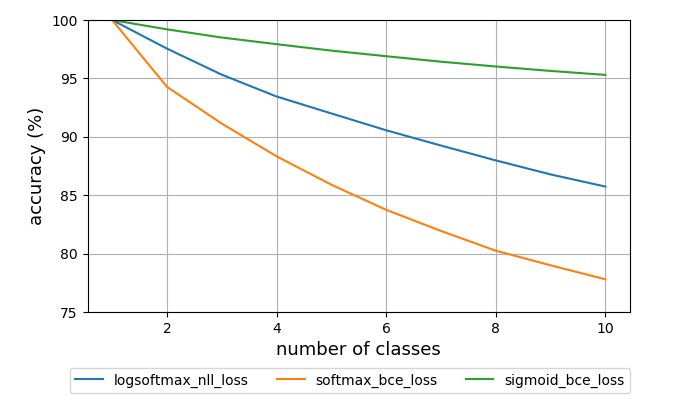
\includegraphics[scale=0.5,trim={0mm 0mm 0mm 0mm},clip]{mnist.png}
    \caption{Accuracy of composed model for MNIST with respect to number of classes}
    \label{figure:composed_mnist}
\end{figure}

\subsection{Keyword Spotting}

To understand the universality of Composing algorithm, I extend this idea to keyword spotting where the input data is audio. The goal of Keyword Spotting (KWS) is to detect an audio of pre-trained keywords, such as “Hey Siri”. Since the first application of deep learning on KWS by~\cite{chen2014small}, Neural network has became standard approach for KWS. In this experiment, I implement \texttt{res15-narrow} introduced by~\cite{tang2018deep}, which achieves accuracy of 94\% for 12 keywords on Google’s Speech Commands Dataset~\cite{speechcommandsdataset}. \texttt{res15-narrow} comprises 6 residual blocks with 19 feature maps where each residual block is composed of bias-free convolutional and batch normalization layer.

As opposed to the previous studies with Google’s Speech Commands Dataset where accuracy is evaluated on 12 keywords, I include all 30 keywords as I am interested in how stable Composing algorithm is with larger number of classes. Following the standard feature extraction process for audio, I first construct Forty-dimensional Mel-Frequency Cepstrum Coefficient (MFCC) frames and stack them using 30ms windows with a 10ms shift. Since the dataset consists of one-second long utterances of each word, the processed input has size of $101\times40$.

Throughout 10 experiments conducted, stochastic gradient descent is used to train both base model and fine-tuned model. Training starts with learning rate of 0.1 but it is decreased to 0.001 by factor of ten at different epochs for each training. Base models are trained for 30 epochs with decrease at 10 and 20th epochs and fine-tuned models are trained for 10 epochs with decrease at 4 and 7th epochs.

Unlike MNIST, it is found type of loss function introduces difference in accuracy for KWS (see Table \ref{table:kws}). \texttt{res15-narrow} achieves the best accuracy when it is trained with CE loss; 93.09\% accuracy from the base model with average accuracy of 95.32\% from fine-tuned models. Softmax with BCE loss achieves 90.94\% accuracy with base model and average accuracy of 91.79\% with fine-tuned models. Sigmoid with BCE loss starts from the lowest accuracy of 89.62\% with fine-tuned models of 91.31\% accuracy.

However, as observed with MNIST, sigmoid with BCE loss shows the least relative decreases from the base model accuracy. While sigmoid with BCE loss leads to relative decrease of 1.44\%, CE loss and softmax with BCE loss shows relative decreases of 3.18\% and 4.57\% respectively. From figure \ref{figure:composed_kws}, it is found that accuracy of composed models decreases again for KWS as number of classes increases.

\begin{table}[t]
    \centering
    \begin{tabular}{ccccccc}
        \toprule[1pt]
        \multirow{2}{*}{\raisebox{-3\heavyrulewidth}{\bf Loss function}} &
        \multirow{2}{*}{\raisebox{-3\heavyrulewidth}{\bf Base model}} &
        \multicolumn{3}{c}{\bf Fine tuned model } &
        \multicolumn{2}{c}{\bf Composed model } \\
        \cmidrule(lr){3-5}
        \cmidrule(lr){6-7}
        & & average & minimum & maximum & accuracy & relative decrease \\
        \midrule
        LogSoftmax + NLL & 93.09 & 95.32 & 92.57 & 97.59 & 90.13 & 3.18 \\
        Softmax + BCE & 90.94 & 91.79 & 89.64 & 94.80 & 86.78 & 4.57 \\
        Sigmoid + BCE & 89.62 & 91.31 & 88.73 & 93.91 & 88.33 & 1.44 \\
        \bottomrule[1pt]
    \end{tabular}
    \caption{Average accuracy of base, fine-tuned, and composed model for KWS}
    \label{table:kws}
\end{table}

\begin{figure}[t]
    \centering
    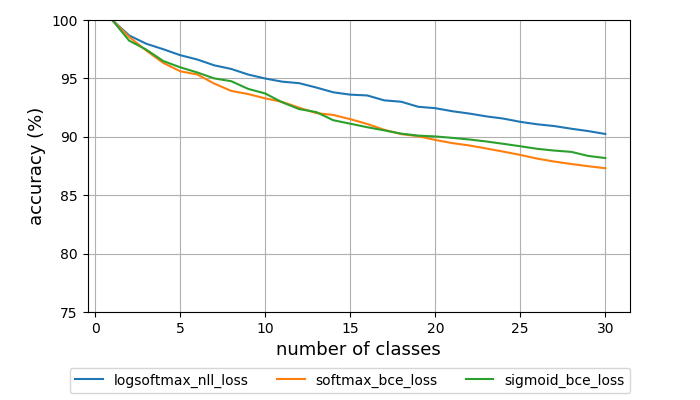
\includegraphics[scale=0.5,trim={0mm 0mm 0mm 0mm},clip]{kws.png}
    \caption{Accuracy of composed model for KWS with respect to number of classes}
    \label{figure:composed_kws}
\end{figure}

\subsection{CIFAR-100}

CIFAR is a collection of tiny colour images from the web introduced by~\cite{krizhevsky2009learning}. There exist two kind of CIFAR varying on number of classes: CIFAR-10 and CIFAR-100. The following experiment is constructed with CIFAR-100 which constitutes of 600 images of 100 classes.

For this experiment, I have implemented \texttt{DenseNet}, a state of the art model architecture for CIFAR dataset~\cite{huang2017densely}. Building upon the architecture with residual connection, the feature maps of all preceding layers are used as inputs for each layer. The network has three dense blocks with transition layers between which changes the feature-map sizes by convolution and pooling. The original implementation achieves accuracy of 80\% with 300 epochs of stochastic gradient descent. Learning rate must decrease throughout the training from 0.1 to 0.001 by factor of ten.

Table \ref{table:cifar} summarizes the accuracy of models throughout Composing algorithm, trained with different loss functions. As training \texttt{DenseNet} for CIFAR-100 is very expensive, only one base model has been trained for each loss functions. However, composing experiments are conducted with 10 iterations, same as the preceding experiments. In this experiment, the base models are trained for 200 epochs achieving accuracy of 69.95\% for CE loss, 64.23\% for softmax with BCE loss, and 64.72\% for sigmoid with BCE loss. Fine-tuned models are trained for 100 epochs with average accuracy of 86.12\%, 88.63\%, and 87.79\% respectively.

\begin{table}[t]
    \centering
    \begin{tabular}{ccccccc}
        \toprule[1pt]
        \multirow{2}{*}{\raisebox{-3\heavyrulewidth}{\bf Loss function}} &
        \multirow{2}{*}{\raisebox{-3\heavyrulewidth}{\bf Base model}} &
        \multicolumn{3}{c}{\bf Fine tuned model } &
        \multicolumn{2}{c}{\bf Composed model } \\
        \cmidrule(lr){3-5}
        \cmidrule(lr){6-7}
        & & average & minimum & maximum & accuracy & relative decrease \\
        \midrule
        LogSoftmax + NLL & 69.95 & 86.12 & 71.00 & 96.00 & 52.74 & 24.60 \\
        Softmax + BCE & 64.23 & 88.63 & 79.50 & 97.50 & 52.04 & 18.98 \\
        Sigmoid + BCE & 64.72 & 87.79 & 77.50 & 96.00 & 57.42 & 11.28 \\
        \bottomrule[1pt]
    \end{tabular}
    \caption{Average accuracy of base, fine-tuned, and composed model for CIFAR-100}
    \label{table:cifar}
\end{table}

\begin{figure}[t]
    \centering
    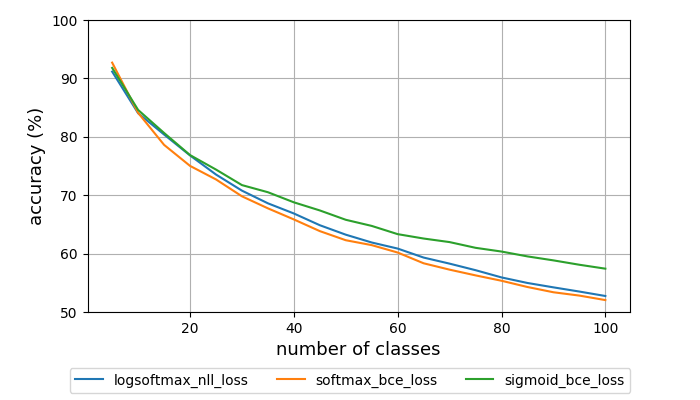
\includegraphics[scale=0.5,trim={0mm 0mm 0mm 0mm},clip]{cifar100.png}
    \caption{Accuracy of composed model for CIFAR-100 with respect to number of classes}
    \label{figure:composed_cifar}
\end{figure}

Figure \ref{figure:composed_cifar} shows how accuracy of composed model changes as number of classes increases. It is found that CIFAR-100 introduces greater rate of relative decrease than MNIST and KWS. I believe this is due to the fact that CIFAR-100 involves much larger number of classes. Again, limitation of CE loss is clear as it leads to 24.60\% relative decrease with respect to the base model accuracy. On the other hand, sigmoid with BCE loss introduces the least relative decrease of 11.28\%.

\section{Conclusion and Discussion}

Realizing the inefficiency with the traditional classifier deployment, I propose Composing algorithm which achieves dynamic construction of a model for an efficient classification adapting to the change in target class set. As loss function plays a key role in Composing algorithm, it is shown both theoretically and empirically that CE loss leads to greater loss of accuracy than sigmoid with BCE loss.

Even though sigmoid with BCE loss leads to minimal decrease in accuracy, it is shown to have strong correlation with the number of classes. In the case of CIFAR-100, it has shown relative decrease of 11.28\% which can be crucial in many cases. Building upon this work, exploring other type of loss such as MSE loss and KL divergence loss would be an interesting study.

Next, proposed Composing algorithm assumes that the last layer is fully-connected. However, some networks apply global averaging as it last operation to minimize computation. I strongly believe that the same approach works for such networks if fine-tuning is achieved for the last convolutional layer.

Overall, I have shown how much flexibility one can achieve for classification by fine-tuning the last fully-connected layer. However, as models involve more and more layers, such flexibility and computational savings may not add much benefit. Therefore, it is necessary extend this idea to save more computations than just last layer, in order for this idea to be meaningful for practical use.

\newpage

\section*{Acknowledgement}
Thank people who have helped or influenced you in this project.

\nocite{*}

\bibliographystyle{unsrtnat}
\bibliography{citation}

\end{document}
